\documentclass[]{article}
% Added package start here
\usepackage{array}
\usepackage{geometry} % for margin of paper
\geometry{margin=1.2in}
\usepackage{fancyhdr} % for headers and footers
\usepackage{graphicx} % for image
\graphicspath{ {media/} }
\pagenumbering{gobble} % Delete page number
% End here
\usepackage{lmodern}
\usepackage{amssymb,amsmath}
\usepackage{ifxetex,ifluatex}
\usepackage{fixltx2e} % provides \textsubscript
\ifnum 0\ifxetex 1\fi\ifluatex 1\fi=0 % if pdftex
  \usepackage[T1]{fontenc}
  \usepackage[utf8]{inputenc}
\else % if luatex or xelatex
  \ifxetex
    \usepackage{mathspec}
  \else
    \usepackage{fontspec}
  \fi
  \defaultfontfeatures{Ligatures=TeX,Scale=MatchLowercase}
\fi
% use upquote if available, for straight quotes in verbatim environments
\IfFileExists{upquote.sty}{\usepackage{upquote}}{}
% use microtype if available
\IfFileExists{microtype.sty}{%
\usepackage{microtype}
\UseMicrotypeSet[protrusion]{basicmath} % disable protrusion for tt fonts
}{}
\usepackage{hyperref}
\hypersetup{unicode=true,
            pdfborder={0 0 0},
            breaklinks=true}
\urlstyle{same}  % don't use monospace font for urls
\usepackage{graphicx,grffile}
\makeatletter
\def\maxwidth{\ifdim\Gin@nat@width>\linewidth\linewidth\else\Gin@nat@width\fi}
\def\maxheight{\ifdim\Gin@nat@height>\textheight\textheight\else\Gin@nat@height\fi}
\makeatother
% Scale images if necessary, so that they will not overflow the page
% margins by default, and it is still possible to overwrite the defaults
% using explicit options in \includegraphics[width, height, ...]{}
\setkeys{Gin}{width=\maxwidth,height=\maxheight,keepaspectratio}
\IfFileExists{parskip.sty}{%
\usepackage{parskip}
}{% else
\setlength{\parindent}{0pt}
\setlength{\parskip}{6pt plus 2pt minus 1pt}
}
\setlength{\emergencystretch}{3em}  % prevent overfull lines
\providecommand{\tightlist}{%
  \setlength{\itemsep}{0pt}\setlength{\parskip}{0pt}}
\setcounter{secnumdepth}{0}
% Redefines (sub)paragraphs to behave more like sections
\ifx\paragraph\undefined\else
\let\oldparagraph\paragraph
\renewcommand{\paragraph}[1]{\oldparagraph{#1}\mbox{}}
\fi
\ifx\subparagraph\undefined\else
\let\oldsubparagraph\subparagraph
\renewcommand{\subparagraph}[1]{\oldsubparagraph{#1}\mbox{}}
\fi

\date{}

\begin{document}
% Added information start here
\pagestyle{fancy}
\renewcommand{\headrulewidth}{0pt}
% footer
  \fancyfoot[L]{\footnotesize This material is based upon work supported by the U.S. Department of Energy Office of Science, Advanced Scientific Computing Research and Biological and Environmental Research programs. \begin{flushright} \footnotesize Version 0.2, April 25, 2016 \end{flushright}}
  
\fancypagestyle{empty}{
% header
\fancyhead[C]{\LARGE {\textbf{What is CSE Software Productivity}}\\ \normalsize {The IDEAS Scientific Software Productivity Project} \\ \small {\href{https://ideas-productivity.org/resources/howtos/}{\emph{ideas-productivity.org/resources/howtos/}}}} 
  \fancyhead[R]{
\includegraphics[width = 3 cm, height = 1.5 cm]{ideas_Whatis}}	
}
\thispagestyle{empty}
\textbf{\newline}
\textbf{\newline}
% Added information ends here.

\textbf{Productivity} is generally a measure of output vs. input. In
most situations we care about increasing quantity or improving quality
of output and reducing cost in time and resources of required input.

\textbf{Scientific Productivity} is concerned with measuring the number
and quality of science results for a research team over a span of time.
If we can measure scientific productivity, we can manage and improve it.

\textbf{CSE Software Productivity:} Computational Science and
Engineering (CSE) Software Productivity is concerned with efforts to
produce, deliver, maintain, and extend software capabilities that make a
science or engineering team more productive. \emph{CSE Software
Productivity improves if scientific and engineering impact improves,
resource costs decrease, solution time is quicker, or a combination of
these three elements improves, attributable to the software.}

\textbf{Extreme-Scale CSE Software Productivity:} Many CSE software
products are required to run on the latest extreme-scale computing
systems. High-fidelity, multiscale, multiphysics simulations with
uncertainty quantification and optimality increase the computing demands
up to and beyond the capability of current leadership systems. At this
scale of computing, the disruption of hardware architecture changes, new
and immature system software environments, and the sheer scope and
complexity of the target problems can be serious impediments to
realizing science and engineering goals. The capabilities of these
systems are the only vehicle for obtaining some important computational
results, but the cost in time and effort can be very high. A focus on
general productivity enhancement is critical at this scale, as is
performance portability.

%\includegraphics[width=4.63229in,height=3.50224in]{media/image03.jpg}
\begin{minipage}{0.7\textwidth}
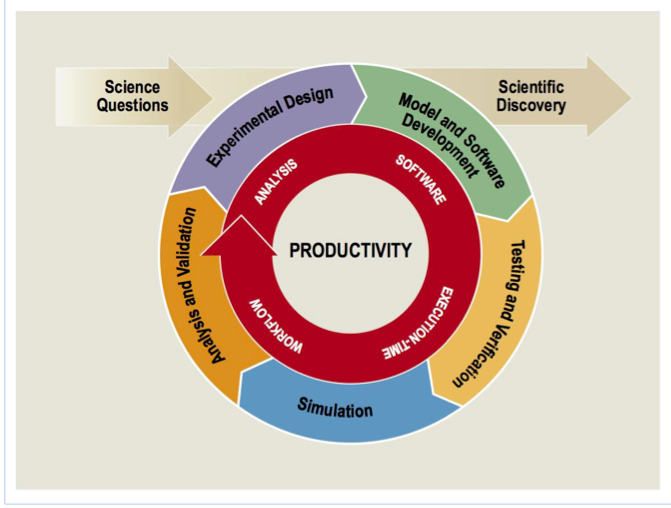
\includegraphics[width=0.8\textwidth]{productivity}
\end{minipage}
\hfill
\begin{minipage}{0.3\textwidth}\raggedright
CSE is broadly recognized as a peer with experimental and theoretical
research in the process of scientific discovery. Improving CSE software
productivity can play a critical and unique role in accelerating the
cycle of scientific discovery on emerging extreme-scale architectures.
\end{minipage}

\textbf{A Practical Characterization of CSE Software
Productivity}

A common saying in product development is, ``Better, faster, cheaper:
Pick two of the three.'' Given a fixed level of productivity, this
saying acknowledges that if product development is behind schedule,
product features must be dropped, the schedule must slip, or more
resources must be applied to the project. At least one of the three must
be adjusted. \emph{Productivity is a volume measure of these three
concerns. CSE Software Productivity is this measure applied to software
developed for and used by scientists and engineers.}

\textbf{CSE Software Productivity Impacts Scientific
Productivity}

\textbf{Solution quality:} The community has many metrics that attempt
to measure the impact of scientific and engineering efforts. CSE
software can improve impact by enabling computer modeling \& simulation,
design optimization, and uncertainty quantification to provide answers
to important science and engineering problems. In some problem domains,
e.g., astrophysics and nuclear stockpile certification, CSE plays a
particularly important role, since theories are incomplete and direct
experimentation is not possible.

\textbf{Time to solution:} CSE software can be used to dramatically
reduce time to solution. CSE simulations can quickly eliminate
infeasible solutions, e.g., in molecular dynamics, or provide unique
insight into system behavior. In advanced environments, CSE software is
used to provide an optimal solution with error bars.

\textbf{Resources:} CSE software can be used to replace or reduce
experimentation costs, e.g., crash simulations. Consequently, people
with good CSE software skills are in high demand, within the scientific
research community and in other industries. Making effective use of
skills and increasing CSE software usability are critically important.

\emph{\textbf{Improving CSE software productivity will improve
scientific productivity.}}

\textbf{Why Focus on CSE Software
Productivity?}

CSE software plays a critical role in science and engineering. At the
same time, the CSE community faces numerous challenges and opportunities
in the coming years:

\textbf{Disruptive hardware changes:} The advent of many-core and
accelerator processors requires a fundamental change in algorithms and
software design.

\textbf{Increased demand for multiscale and multiphysics coupling:}
These same disruptive hardware changes provide dramatic growth in
computational capabilities. These capabilities enable scientists to
consider coupled simulations, which, in turn, demand that multiple CSE
software packages be used in combination to solve a single problem.

\textbf{Increased opportunities to incorporate computation into
projects:} CSE software has proven effective in solving many problems,
and its impact can spread -\/- if we develop the software capabilities.

\textbf{Limited staff resources in high demand:} The skill set for
developing CSE software is large, including domain knowledge,
mathematics, and computer science. For larger projects, effective team
skills are also required. Furthermore, parts of this skill set are in
high demand in other areas of the economy, resulting in a shortage of
skilled people.

An explicit focus on software productivity will help computational
scientists and engineers address challenges and opportunities by
providing a toolset, methodologies, and information to better manage
large, complex, and rapidly changing software systems while delivering
higher-quality results faster, with fewer resources.

This document was prepared by Michael A. Heroux with key contributions
from Hans Johansen, David Bernholdt and Lois Curfman McInnes.

\end{document}
